\documentclass[12pt, a4paper, twoside]{article}
\usepackage[utf8]{inputenc}
\usepackage[cm]{fullpage}
\usepackage{fancyhdr}
\usepackage{textcomp}
\usepackage{graphicx}
\usepackage{commath}
\usepackage[portuguese]{babel}
\usepackage{float}
\usepackage{hyperref}

\title{Pré-experimento 6 de LDCE}
\author{Cris Joe Silva Jr.}
\date{\today}

\begin{document}

\maketitle

\section{Introdução}

Neste relatório, utilizaremos o modelo descrito na figura 1 para o transistor NPN.

\begin{figure}[H]
    \centering
    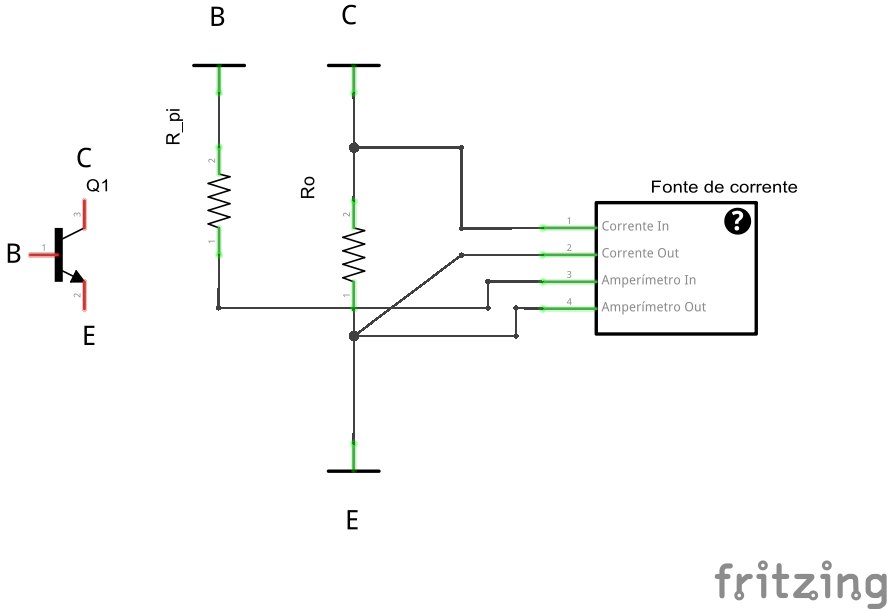
\includegraphics[width=0.8\textwidth]{figs/bjt.png}
    \caption{Modelo do transistor de junção bipolar do tipo NPNr.}
\end{figure}


\section{Questionamentos}

\subsection{Questão 1}

O \textit{BC548} se caracteriza por ser um transistor de uso geral mas com especificações de tensão e corrente grandes o suficiente para ser utilizado como um dispositivo de eletrônica de potência. Já o \textit{BC338} é um transistor com especificações mais próprias para baratear sistemas de sinal, se tornando impróprio como transistor de potência.

\subsection{Questão 2}

O transistor \textit{TIP31} é um transistor NPN, enquanto o transistor \textit{TIP32} é um transistor PNP. Fora isso, todas as suas especificações técnicas são equivalentes. Contudo, eles não podem ser utilizados intercambiavelmente por funcionarem de maneira complementar.

\subsection{Questão 3}

\begin{figure}[H]
    \centering
    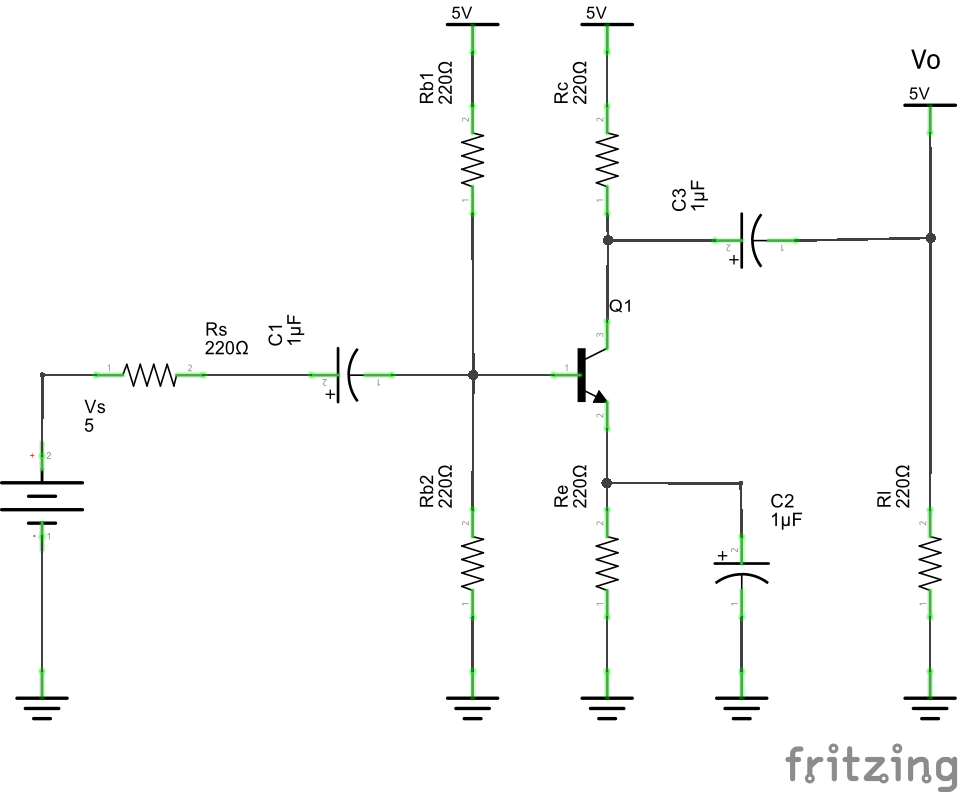
\includegraphics[width=0.6\textwidth]{figs/rel6/circuit.png}
    \caption{Circuito a ser analisado neste pré-relatório.}
\end{figure}

Para descobrir o circuito equivalente AC do problema em questão, podemos:

\begin{enumerate}
    \item Remover as fontes DC do circuito;
    \item Substituir o transistor pelo seu modelo.
\end{enumerate}

Se considerarmos que os capacitores $C_1$, $C_2$ e $C_3$ tiverem capacitâncias altas o suficiente em relação às frequências do circuito, podemos substituí-los por curtos. Neste caso, o circuito equivalente se torna o circuito da figura 3.

\begin{figure}[H]
    \centering
    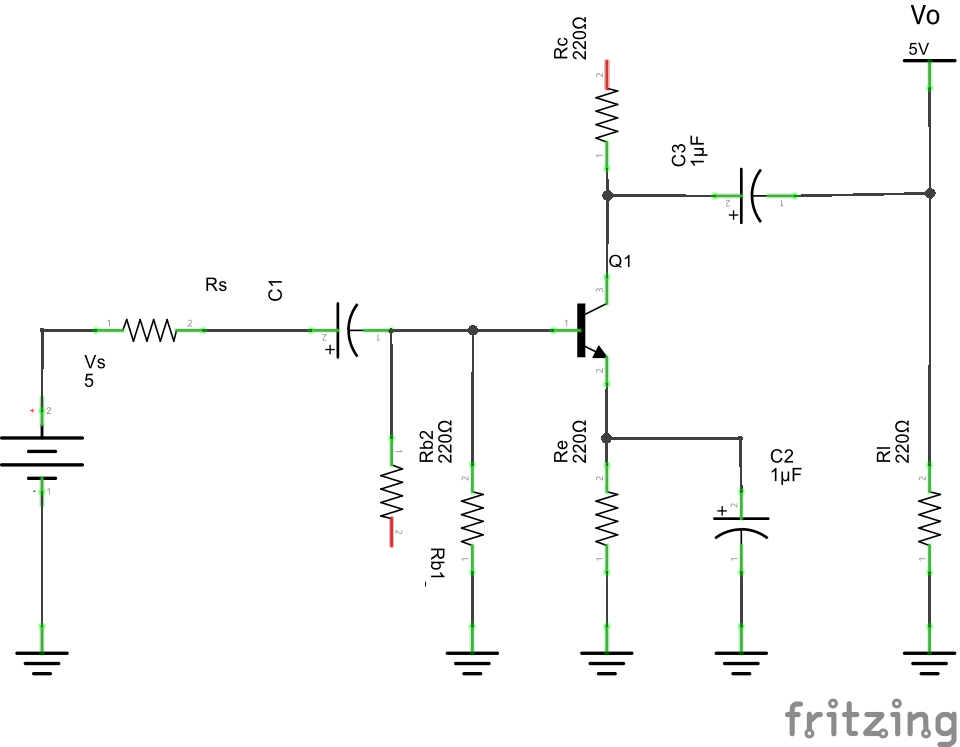
\includegraphics[width=0.6\textwidth]{figs/rel6/ac_eq.png}
    \caption{Circuito AC equivalente do circuito da figura 2.}
\end{figure}

\subsection{Questão 4}

\begin{figure}[H]
    \centering
    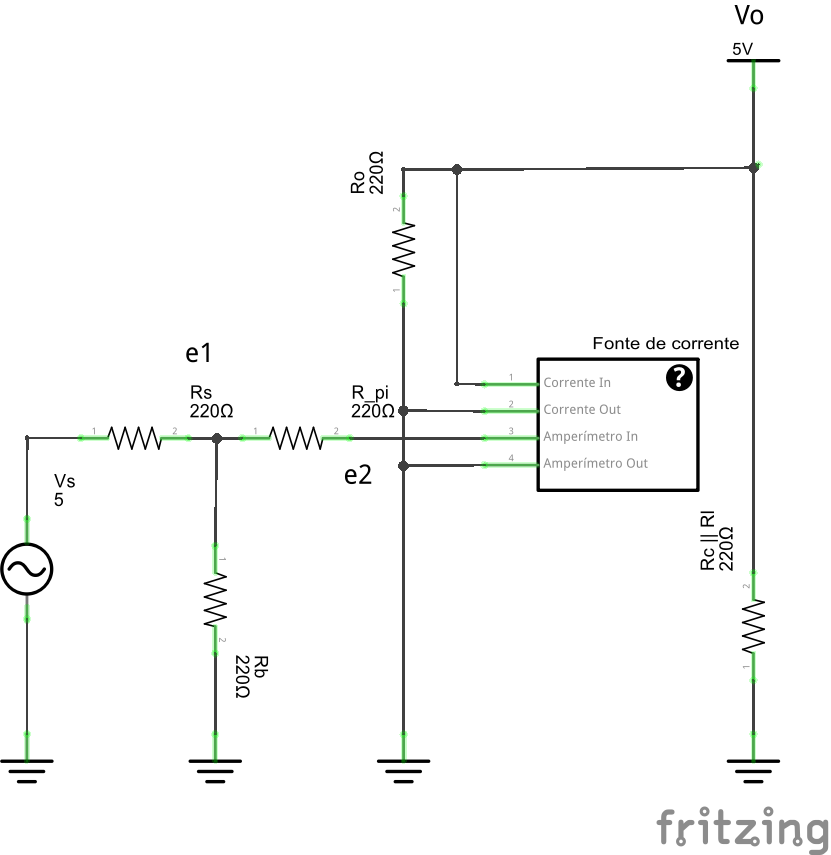
\includegraphics[width=0.6\textwidth]{figs/rel6/ex4.png}
    \caption{Circuito a ser analisado neste pré-relatório.}
\end{figure}

Para descobrir $v_o$, podemos aplicar a lei de Kirchhoff das correntes no circuito e analisar sua montagem. Inicialmente vamos definir $ R_B := R_{b1} || R_{b2} $. Em seguida, vamos definir os nós $e_1$ e $e_2$. Aplicando a lei de Kirchhoff das correntes, temos,

\begin{equation}
    \begin{cases}
        \frac{V_S-e_1}{R_S} = \frac{e_1 - 0}{R_B} + \frac{e_1-e_2}{r_\pi} \\
        \frac{e_1-e_2}{r_\pi} + \beta i_B = \frac{e_2 - v_o}{r_o} \\
        \beta i_B + \frac{v_o - 0}{R_C||R_L} = \frac{e_2 - v_o}{r_o}
    \end{cases}
\end{equation}

Da montagem do circuito, temos que
$$ e_2 = 0 $$
$$ i_B = \frac{e_1 - e_2}{r_\pi} = \frac{e_1}{r_\pi} $$

Resolvendo o sistema para $V_S$, $e_1$ e $v_o$, temos que
$$ v_o(t) = -V_S(t) \cdot \frac{r_o}{r_\pi} \cdot (1+\beta) \cdot \frac{1}{R_S} \cdot \left(\frac{1}{R_S} + \frac{1}{R_B} + \frac{1}{r_\pi} \right)^{-1} $$

\subsection{Questão 5}

Pela definição,
$$ A_v = \frac{v_o}{v_i} = \frac{v_o(t)}{V_S(t)} = \frac{r_o}{r_\pi} \cdot (1+\beta) \cdot \frac{1}{R_S} \cdot \left(\frac{1}{R_S} + \frac{1}{R_B} + \frac{1}{r_\pi} \right)^{-1} $$

\subsection{Questão 6}

% TODO Simular circuito.

\subsection{Questão 7}

A saída de um circuito é do tipo \textit{push-pull} quando ela não pode ser dividida com a saída de outros circuitos. É a saída geralmente utilizada em circuitos digitais a fim de facilitar o projeto de um sistema mais complexo.

\section{Referência Bibliográfica}

\begin{itemize}
    \item TODO Add datasheets
\end{itemize}

\end{document}
